\section{Results}\label{sec:results}

\subsection{N2: reconstruction on the live web}\label{sec:results-n2}

N2 ran three experiments. E-LIVE checks that the pipeline runs on the live web without fabricating
or mislabeling; it has no gold and no threshold. E-PLANT and E-ABST are pre-registered, gated
experiments that compare the gated pipeline with an ungated raw model.

\paragraph{E-LIVE.} \evobs{} Two domains ran with the same models: PLC intermittent-fault diagnosis
(technical, procedural) and GDPR data protection impact assessments (legal, normative). A post-fix PLC
rerun crashed on a PDF encoding defect (0 claims). \Cref{tab:elive} gives the completed
runs.\footnote{\repo{research/n2/e_live_report.md}, \S3 and \S5; recomputed from each run's
\code{sidecar.json} and \code{ledger.json}.}

\begin{table}[htbp]
  \centering\small
  \caption{E-LIVE per-run counts. \enquote{Unknown claims} are slots searched, fetched and fully
    verified with nothing found. GDPR v2 is defect-compromised: 140 of its 366 evidence items kept a
    pending verdict after silent verifier failures, so it is not admissible for N3.}
  \label{tab:elive}
  \begin{tabularx}{\linewidth}{@{}Xrrrrrr@{}}
    \toprule
    Run & Sources & Extracted & Located & Verified & Unknown claims & Cost \\
    \midrule
    PLC v1 & 35 & 370 & 337 & 321 & 5 & \$0.679 \\
    GDPR v1 & 20 & 259 & 204 & 195 & 14 & \$0.500 \\
    GDPR v2 (not admissible) & 25 & 523 & 351 & 207 & 15 & \$1.002 \\
    \bottomrule
  \end{tabularx}
\end{table}

\evobs{} \emph{Exact spans.} All 909 evidence items of the three ledgers re-slice exactly from their
snapshots (337 + 206 + 366); a separate sample of 71 re-sliced 71 of 71, checked by an AI inspector,
not a human. The claims are a different matter: of 1,169 claims, 418 are labeled
\code{synthetic_extrapolation} (49, 64 and 305) and 34 \code{unknown}, so 452 (39\%) have no supporting
span. \emph{Verifier error.} On sampled claims the verifier's main error is scope drift, not
fabrication: 30\% on PLC v1 (Wilson 95\% CI 15--52\%, $n = 20$) and 12\% on GDPR v2 (4--30\%,
$n = 25$, in-sample). GDPR v1's 14 unknown slots concentrate in \code{failure_mode} (5 of 5 areas):
regulator text states obligations, not how an assessment goes wrong in practice; \evint{} this fits the
kind of gap the gap map targets, but it is not validated.

\evobs{} \emph{Decoys.} Supported claims were mutated (negation, a changed number or scope) and checked
again against the original span. The verifier accepted 7 of 20 decoys on PLC v1 (35\%, 18--57\%) and 3
of 20 on GDPR v1 (15\%, 5--36\%). Three PLC scope decoys only dropped a conjunct, so the span still
entailed them; without them the rate is 4 of 17 (24\%, 10--47\%). \evint{} The label
\code{literature_supported}, which every lens reads, rests on a verifier that accepted between a quarter
and a third of mutated PLC claims. A false \enquote{supported} claim can seed a gap candidate.

\evobs{} \emph{Defects found live.} Running on the real web surfaced eleven defects that 416 passing
offline tests had missed, among them verifier failures hidden behind a \code{complete: true} flag
(Extended Technical Report, Appendix~D). None of the fixes was re-checked live, and the current cross-verify and decoy stages have
never run live.

\paragraph{E-PLANT and E-ABST.} E-PLANT gives the raw model a false planted value among about 12 real
pages that state the truth, and asks whether it repeats the plant. Its validity floor assumed the
ungated model would adopt plants on more than 60\% of targets, a figure taken from ClashEval
\parencite{wu2024clasheval}. That figure holds only for two models, with the planted document as the only
context, a condition E-PLANT did not reproduce. E-ABST asks the raw model real but private questions and
counts false answers where it should abstain.

\begin{evobsbox}[unbreakable]
  \textbf{N2's registered verdict: INCONCLUSIVE.} The ungated model adopted $a_U = 5$ of 24 plants
  (21\%, Wilson 9--40\%), below the registered validity floor of 8. By the pre-registered rule this
  closed the Continue route before any gated arm was scored; it is a result about the test's
  sensitivity, not about gating. In E-ABST the raw model answered only 5 of 24 private items and
  abstained on 19 (79\%), so the required 20-point margin was reachable only in a narrow corner. The
  gated arms were never scored. \textbf{No statement about whether gating reduces planted falsehoods or
  false answers is supported.}
\end{evobsbox}

\evobs{} \emph{Budget stop.} N2's total spend was about \$4.82 against a \$5 weekly key limit (E-LIVE
\$2.374, E-PLANT \$1.953, E-ABST \$0.495), while the three experiments' registered caps summed to about
\$21. The post-fix live re-check (E-LIVE v3) stopped at its first call on the provider's key limit.
The owner chose not to raise it. \evint{} Budget headroom is part of the design: limits must be checked
against the sum of caps before a run sequence starts, and a \enquote{beats the baseline} gate must be
calibrated on a pilot before it is registered.

\subsection{N3: the gap map}\label{sec:results-n3}

\paragraph{Lenses.} \evobs{} Seven lenses fire over criterion-labeled claims only. They read the
extractor's paraphrase of each claim, not the verbatim span, and three of them depend on knowledge types
the extractor assigned. Lens firing tracks domain texture as designed: DIAG fires only on PLC, the
diagnostic domain; DISC and HEDGE fire mainly on GDPR, the normative one (\cref{tab:firing}). This shows
that lenses distinguish texture, not that they find hidden knowledge.

\begin{table}[htbp]
  \centering\small
  \caption{Lens firing per ledger. \enquote{Promotional excluded} counts candidates dropped before
    judgment by a domain denylist tuned in-sample.}
  \label{tab:firing}
  \begin{tabularx}{\linewidth}{@{}lrXr@{}}
    \toprule
    Ledger & Fired & By lens & Promotional excluded \\
    \midrule
    PLC & 56 & WHY 24, RESULT 19, DIAG 9, SEL 2, DISC 1, GUARD 1 & 42 \\
    GDPR v1 & 51 & RESULT 21, DISC 13, WHY 8, HEDGE 5, SEL 4 & 8 \\
    GDPR v2 & 48 & DISC 14, SEL 11, RESULT 9, WHY 9, HEDGE 5 & 1 \\
    \bottomrule
  \end{tabularx}
\end{table}

\paragraph{The absence check.} A fired lens only shows that a construct is named. Deciding that its
content is really \emph{unsaid} is the absence check. The PoC tried two versions.

\evobs{} \emph{Lexical closure} scored a candidate closed if another claim shared enough word stems.
Against a null of 200 random-donor draws, the observed closure counts fall within or below the null's
5--95\% interval on every ledger: PLC 22 against a null mean of 33.48 (26--41), GDPR v1 11 against
12.735 (8--17), GDPR v2 11 against 8.08 (5--12). Lexical closure did no better than chance.

\evobs{} \emph{Semantic closure}, the final version, asks the local judge to decide from retrieved
sentences whether the missing element is \code{closed}, \code{partial} or \code{open}. The fair control
keeps the seed's own sentences in both arms and swaps only the other-source sentences for those of the
topically nearest candidate of the same lens. Counting \code{partial} as closed, the judge's rate is the
same in both arms: \textbf{PLC 0.889, GDPR v1 0.961, GDPR v2 0.958} ($n = 54, 51, 48$). Every tested
lens in every ledger is flagged \code{closure-uninformative} (\cref{fig:closure}).\footnote{Each
\code{research/n3/*/gapmap.json}, field \code{checks.mismatched_evidence_control}.}

\begin{figure}[tbp]
  \centering
  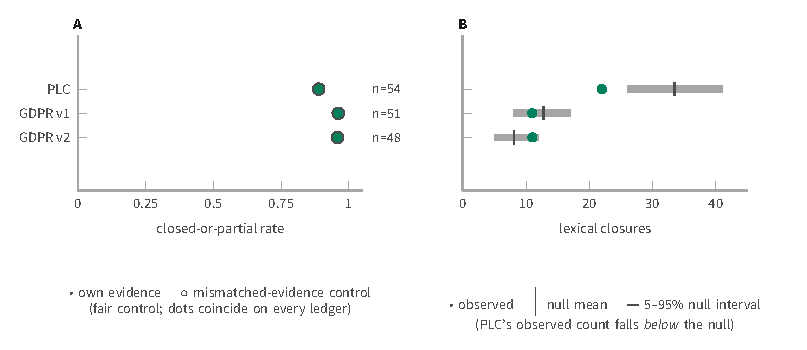
\includegraphics{figures/pdf/fig08_closure.pdf}
  \caption[The absence check versus its fair control]{Does the absence check beat its fair control?
    It does not. Panel~A: closed-or-partial rate on a candidate's own evidence and on the fair control,
    by ledger; the rates are equal. Panel~B: observed lexical closures against the donor null (mean and
    5--95\% interval of 200 draws).}
  \label{fig:closure}
\end{figure}

Four qualifications keep this in proportion. In 32 of the 153 pairs the two arms sent the judge an
identical prompt, so equality there holds by construction. Counted on \code{closed} alone, own versus
control is 0.30/0.33, 0.65/0.61 and 0.58/0.52, still far below the 0.20 difference the check requires.
The own rate is 1.0 on 11 of the 14 tested lens--ledger cells, so the test has little room. And an arm
with the seed's sentences removed still closes or partly closes 0.667, 0.725 and 0.708 of candidates,
which fits a lenient judge. \evint{} The reading is narrow: the judge's verdict does not depend on which
evidence it is shown. Every candidate reads \enquote{a lens fired here}, not \enquote{experts know
something here}. \evobs{} An adversarial AI review of the pre-final maps found this weakness; the first
built-in control had been a straw man that \enquote{passed}. The fair control now runs on every replay.

\needspace{5\baselineskip}
\paragraph{Triage, ranking and the display cap.} \evobs{} An unclosed firing becomes a retrieval gap
(\code{RG-UNK}: nothing found; \code{RG-SINGLE}: one independent source; \code{RG-UNVER}: closed only by
unverified text; \code{RG-SIBLING}: closed in a sibling run; \code{RG-UNDECIDED}: unreadable judge
answer), whose action is more search, or a gap candidate (\code{HYP}): an \code{open} or \code{partial}
record with at least two independent sources. A HYP record has three tiers: observed evidence, the
inferred gap, and a hypothesis whose label is fixed to \code{inferred}. Candidates are ranked by a
breadth rubric (independent sources, step breadth, penalties for \code{partial} and promotional seeds),
not by expected information gain. After merging near-duplicates, a display cap keeps at most 12 records,
3 per lens and 4 per area. On PLC it hides 15 of 24 merged candidates (10 RESULT, 5 WHY). Questions are
filled from fixed templates with up to two verbatim quotes; no model writes them.

\begin{table}[htbp]
  \centering\small
  \caption{Final map counts. GDPR v2 is shown only for the cross-run check. RG-UNK is a different
    quantity from N2's unknown claims (\cref{tab:elive}).}
  \label{tab:n3counts}
  \begin{tabularx}{\linewidth}{@{}>{\raggedright\arraybackslash}p{3.4cm}
      >{\raggedright\arraybackslash}X>{\raggedright\arraybackslash}X
      >{\raggedright\arraybackslash}X@{}}
    \toprule
    & PLC & GDPR v1 & GDPR v2 (not admissible) \\
    \midrule
    HYP after merge (uncapped) & 24: RESULT 13, WHY 8, DIAG 2, GUARD 1 & 1: RESULT &
      6: RESULT 3, DISC 1, HEDGE 1, WHY 1 \\
    HYP shown after the cap & 9: RESULT 3, WHY 3, DIAG 2, GUARD 1 & 1 & 6 \\
    Closure state of shown HYP & 3 open, 6 partial & 1 partial & 6 partial \\
    RG-SINGLE / UNVER / SIBLING / UNK & 11 / 0 / n/a / 10 & 12 / 4 / 2 / 28 & 3 / 6 / 7 / 44 \\
    \bottomrule
  \end{tabularx}
\end{table}

\begin{figure}[tbp]
  \centering
  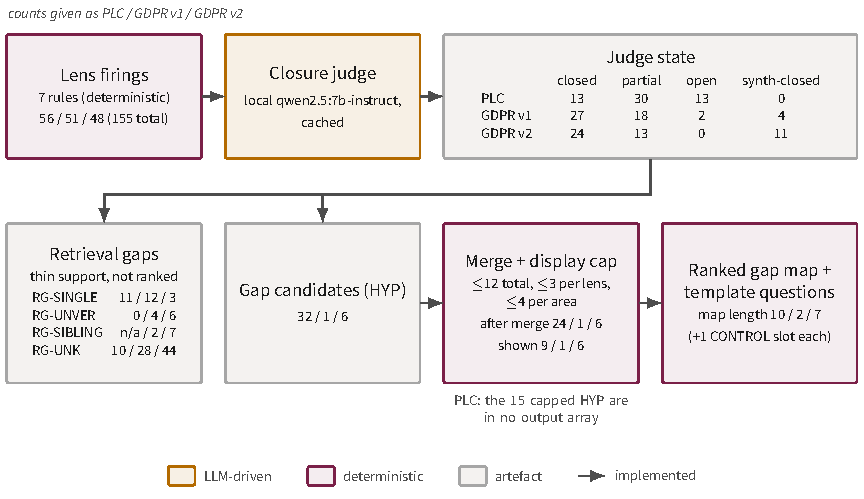
\includegraphics{figures/pdf/fig07_n3.pdf}
  \caption[From lens firing to gap candidate or nothing]{How lens firings become retrieval gaps, gap
    candidates or nothing, with counts per ledger (PLC / GDPR v1 / GDPR v2). After triage, near-duplicate
    HYP records are merged (PLC 24) and a display cap keeps at most 12 (PLC 9 shown). Most shown
    candidates are \code{partial}, not \code{open}.}
  \label{fig:n3}
\end{figure}

\needspace{6\baselineskip}
\paragraph{The negative results, stated plainly.}
\begin{itemize}[nosep]
  \item \evobs{} \textbf{13 of the 16 displayed candidates are \code{partial}.} The two PLC DIAG records
    read \code{open} only because the DIAG rule counts a partially signed rival cause as unsigned; only
    one displayed candidate (PLC rank~7, a WHY record) has no partial hit. \evint{} The fair control
    counts \code{partial} as closed, so most surviving hypotheses sit in a state the map's own control
    would call closed.
  \item \evobs{} \textbf{Precision by adversarial judgment: 3 of 19 strict (8 of 19 lenient), on the
    pre-final maps only} (Wilson 5.5--37.6\% and 23.1--63.7\%). One AI reviewer judged in-sample, with no
    human coder and no gold; the per-record tally is not committed, and the final maps were not
    re-tallied. It is a sanity signal, never a measured precision.
  \item \evobs{} \textbf{PLC's ranking follows source density} (Spearman $\rho = 0.91$; overlap of the
    top ten with the ten highest-density candidates $J_{10} = 0.58$). The anti-renaming check tests only
    the low-density direction ($J_{10} = 0.00$). On GDPR, $\rho$ is 0.09 and 0.16.
  \item \evobs{} \textbf{Cross-run stability is low.} Of GDPR v1's 13 unclosed lens records, 3 have a
    counterpart in the independent v2 run; of v2's 9, 3 have one in v1. Every counterpart is partial.
    \evint{} The runs are dominated by different sources, so the instability traces to retrieval.
  \item \evobs{} \textbf{A judge-parsing defect was found by review, not by tests.} Unparsed judge
    answers had silently defaulted to \code{open} (reported as 24 of 103, 62 of 150 and 60 of 147
    responses). The tests used a fake judge that always answered in format. Unparsable answers now
    become \code{RG-UNDECIDED}.
\end{itemize}

\subsection{One complete trace, and its weaknesses}\label{sec:trace}

\Cref{fig:trace} follows PLC's top-ranked record from source to question. The seed span, from a public
troubleshooting page, reads \enquote{Loose terminals cause many intermittent faults. A flashlight reveals
problems in dark panels that you miss otherwise.} The claim is \code{literature_supported}. Seven
independent sources discuss the topic, and the DIAG lens found five rival causes (ground loops,
aliasing, installation versus software, VFD/contactor noise, pull-up/clock timing). Of 34
verified sentences retrieved, the judge found none that fully states a sign separating any rival, and it
marked 5 claims as partial. The DIAG rule counts a partially signed rival as unsigned, so the record
reads \code{open}. The template question asks: \enquote{Which cause did you suspect first, and what did
you see, hear or measure that let you rule the others out?}, to be asked as CDM probes on a recalled
case, then contrasting cases.\footnote{\repo{research/n3/plc/gapmap.json}, \code{map[0]}, gap
\code{g-59164a9db5bd}.}

\evobs{} \emph{Weaknesses.} The trace was chosen by the author after the maps were final (the
top-ranked record of each map). The question's anchor is the extractor's assertion cut at 80
characters, so the question is not a grammatical sentence. The hypothesis template says the judge
\enquote{found a sign for the following} and then marks every item \enquote{(no sign found)}. The
\code{open} state overstates the evidence, since the judge found partial signs. PLC's second record
repeats the fragment defect, with rival causes such as \enquote{array subscript out of range.} Such a
candidate should not reach an interview unedited. \evint{} The trace shows that the mechanism runs from
a real span to a fixed-frame question, and where model-written text enters. It cannot show, without a
human answer, that the question would surface knowledge a practitioner holds.

\begin{figure}[p]
  \centering
  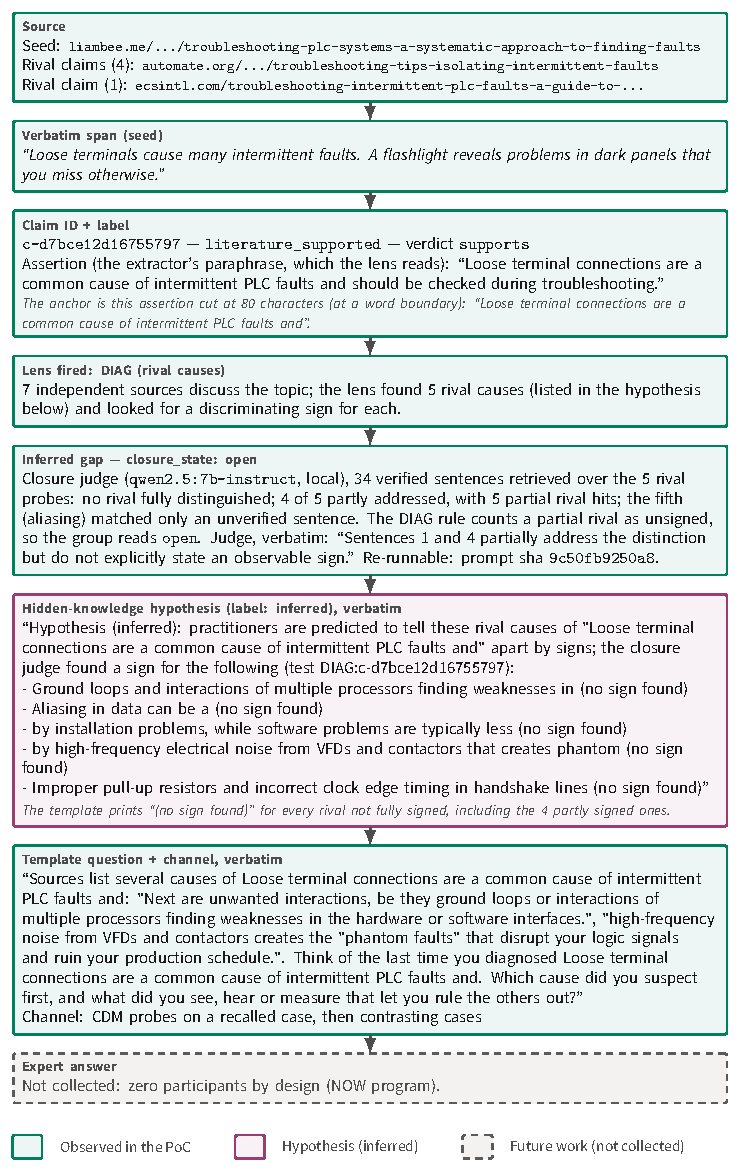
\includegraphics{figures/pdf/fig09_trace.pdf}
  \caption[One complete trace, source to question]{One complete real trace, end to end: seed span and
    claim, DIAG lens with five rival causes, the closure judge's verdict (no rival fully signed; 5 claims
    partly signed, counted as unsigned, so the record reads \code{open}), the hypothesis and the template
    question. The lens fired; the absence check found the element at most partly stated. No expert has
    answered the question.}
  \label{fig:trace}
\end{figure}
